\documentclass[a4paper]{jpconf}
\usepackage{graphicx}
\usepackage{hyperref}
\usepackage{float}

\begin{document}
\title{Deep learning for inferring cause of data anomalies}

\author{V~Azzolini$^1$, M Borisyak$^{2,3}$, G~Cerminara$^4$, D Derkach$^{2,3}$, G~Franzoni$^4$, F~De~Guio$^5$, O Koval$^{6,3}$, M~Pierini$^4$, A~Pol$^7$, F Ratnikov$^{2,3}$, F~Siroky$^4$, A~Ustyuzhanin$^{2,3}$ and J~R~Vlimant$^8$}

\address{$^1$ Massachusetts Institute of Technology, Cambridge, USA \\
$^2$ National Research University Higher School of Economics,  Moscow, Russia \\
$^3$ Yandex School of Data Analysis, Moscow, Russia \\
$^4$ CERN, European Organization for Nuclear Research, Geneva, Switzerland \\
$^5$ Texas Tech University, Lubbock, USA \\
$^6$ Skolkovo Institute of Science and Technology, Moscow, Russia \\
$^7$ University of Paris-Saclay, Paris, France \\
$^8$ California Institute of Technology, Pasadena, USA}

\ead{fratnikov@hse.ru}



\begin{abstract} 
Daily operation of a large-scale experiment is a resource consuming task, particularly from perspectives of routine data quality monitoring. Typically, data comes from different channels (sub-detectors or other subsystems) and the global quality of data depends on the performance of each channel. In this work, we consider the problem of prediction which channel has caused anomalies in the detector behaviour.
We introduce a generic deep learning model and prove, that, under reasonable assumptions, the model learns to identify 'channels' which are affected by an anomaly. Such model could be used for data quality manager cross-check and assistance and identifying good channels in anomalous data samples.
The main novelty of the method is that the model does not require ground truth labels for each channel, only global flag is used. This effectively distinguishes the model from classical classification methods. Being applied to CERN CMS data,  this approach proves its ability to decompose anomaly by separate channels. 
\end{abstract}




\section{Introduction}
Data quality monitoring is a crucial task for every large scale High Energy Physics experiment.
The challenge is driven by the huge amount of data. Considerable amount of person power
required for monitoring and classification. Previously, we designed the system [1], which automatically classifies marginal cases in general: both of 'good' an 'bad' data, and use human expert decision to classify remaining “grey area” cases. 

Typically, data comes from different sub-detectors or other subsystems, and the global data quality depends on the performance of each such channel. In this work, we consider the next type of problem, to predict which sub-detector is responsible for anomaly in the detector behaviour, knowing only global flag. A proposed system can indicate affected channels and draw the attention of human experts to the other channels, as maybe data from them is still useful.




\section{Data and feature extraction}
In these proceedings we use data collected by the CMS experiment [2] at LHC in CERN. Data preprocessing procedure is the same as in the previous work [1], detailed description is presented there. 

All data is divided into chunks - LumiSections, which are labelled as 'good' or 'bad'. Information from four channels (muons, photons, Particle Flow jets or calorimiter jets) for each LumiSections is used. Objects are quantiled by their momentum to have fixed number of features in each event. Then every selected object is characterized by its reconstructed physics properties: mass, spatial location, kinematics. And statistics for each feature for the entire lumisection is computed (5 percentiles, mean and variance).

Additionally as features for the following analysis
scalar sum of momentum for all objects in the event,
instant luminosity and number of particles in event are added.




\section{Method}
In order to predict a probability of anomaly in different sub-detectors separately 
we build a special ‘multi-head’ neural network configuration (figure 1). 

NN consist of four branches and each sub-networks has in input features from 
corresponding channel. Each branch returns a score for its channel. At the end, sub-networks are
connected and the whole network is trained to recover global labels.

As network connection operator logistic regression and min operator with dropout could be used. In this proceedings we present results when sub-networks are connected with kind of 'Fuzzy AND' operator: \begin{eqnarray}
\exp [\sum_{i=1}^4(f_{i} - 1)],
\end{eqnarray}
where $f_{i} - $ is an output of the last layer of sub-networks. It is proved for this operator, that under reasonable assumptions, the model learns to identify 'channels' which are affected by an anomaly.\footnote{The code of the systems with different operators for network connection and prof for 'Fuzzy AND' operator decomposition properties are available at \url{https://github.com/yandexdataschool/cms-dqm/} }

\begin{figure}[h!]
\begin{center}
\includegraphics[width=5in]{figures/net.png}
\end{center}
\caption{\label{label}NN architecture with four sub-networks for each channel}
\end{figure}


The main feature is that proposed approach uses only aggregated global quality tag for training, but allows predicting anomalies for separate channels.

In this way, each subnetwork returns score:
\begin{itemize}
\item close to 1 for good lumisections,
\item close to 1 for anomalies “invisible” from subnetwork’s channel data,
\item close to 0 for anomalies “visible” from subnetwork’s channel data.
\end{itemize}

Thus NN decomposes anomalies by channels.


'Fuzzy AND' approach assumes that there are anomalies not seen from all channels. It is desired setting, but it causes a problem of small gradients during training for close to the hyperplane samples, which are potentially visible from particular channel, but already with negative labels from other channels. Just cross-entropy loss for 'Fuzzy AND' output of the whole network is not sensitive enough in such cases. To resolve the problem and to accelerate the convergence we use a dynamic loss function:
\begin{eqnarray}
L' = (1-C) \cdot L + C \cdot (L_1 + L_2 + L_3 + L_4)/ 4 ,
\end{eqnarray}
where $L - $cross-entropy loss for 'Fuzzy AND' output of the network; $L_i - $ so called 'companion' losses, cross-entropy of corresponding sub-network scores against global labels; $C - $ decreasing along iterations constant to regulate amount of 'pretraining'.

With such 'soft pretraining' dynamic loss function we can force sub-networks to be more accurate and to take care about ambiguous samples during the first training iterations, but then to pay more attention to the predictive power of the whole NN against global labels. Thus, simple enough separation hyperplane is constructed during training, and problem of small gradients, which is mentioned above, is avoided.

\section{Results and discussions}
Being applied to CERN CMS data, method proves its ability to decompose anomaly by separate sub-detectors. In figure 2 distributions of predictions in each NN branch are shown. As expected, we can see scores close to one for 'good' samples. And 'bad' data has two options, it could be visible from channel (score close to zero) or not. We can think about the second cases, as data is not affected by an anomaly and maybe it is still useful for for further physical analysis.

Thus, method suggests that most of anomalies are caused (or at least best detected) by calo channel and there is some of data from others channels, which does not look like like anomalous and can be saved.

In these experiments global predictive power of the whole network is rather high, ROC AUC score equals to 0.96.
To verify obtained results we calculate correlations between sub-network predictions and experts' labels for CMS subsystems, which were not used for training (figure 3). All ROC AUC scores a higher than 0.5, it means that there is a clear correlation between sub-networks’ outputs and corresponding subsystem labels or some of them are almost independent. But there is no anti-correlations, as it is expected.

\begin{figure}[H]
\begin{minipage}[h!]{0.47\linewidth}
\center{\includegraphics[width=14pc]{figures/calo.png}} \\a) 
\end{minipage}
\hfill
\begin{minipage}[h!]{0.47\linewidth}
\center{\includegraphics[width=14pc]{figures/PF.png}} \\b)
\end{minipage}
\vfill
\begin{minipage}[h!]{0.47\linewidth}
\center{\includegraphics[width=14pc]{figures/muons.png}}\\ c) 
\end{minipage}
\hfill
\begin{minipage}[h!]{0.47\linewidth}
\center{\includegraphics[width=14pc]{figures/photons.png}} \\ d) 
\end{minipage}
\caption{Distributions of predictions returned by NN branches build on features from a) calorimiter, b) particle flow jets, c) muons, d) photons
channels.}
\label{ris:experimentalcorrelationsignals}
\end{figure}


\begin{figure}[H]
\begin{center}
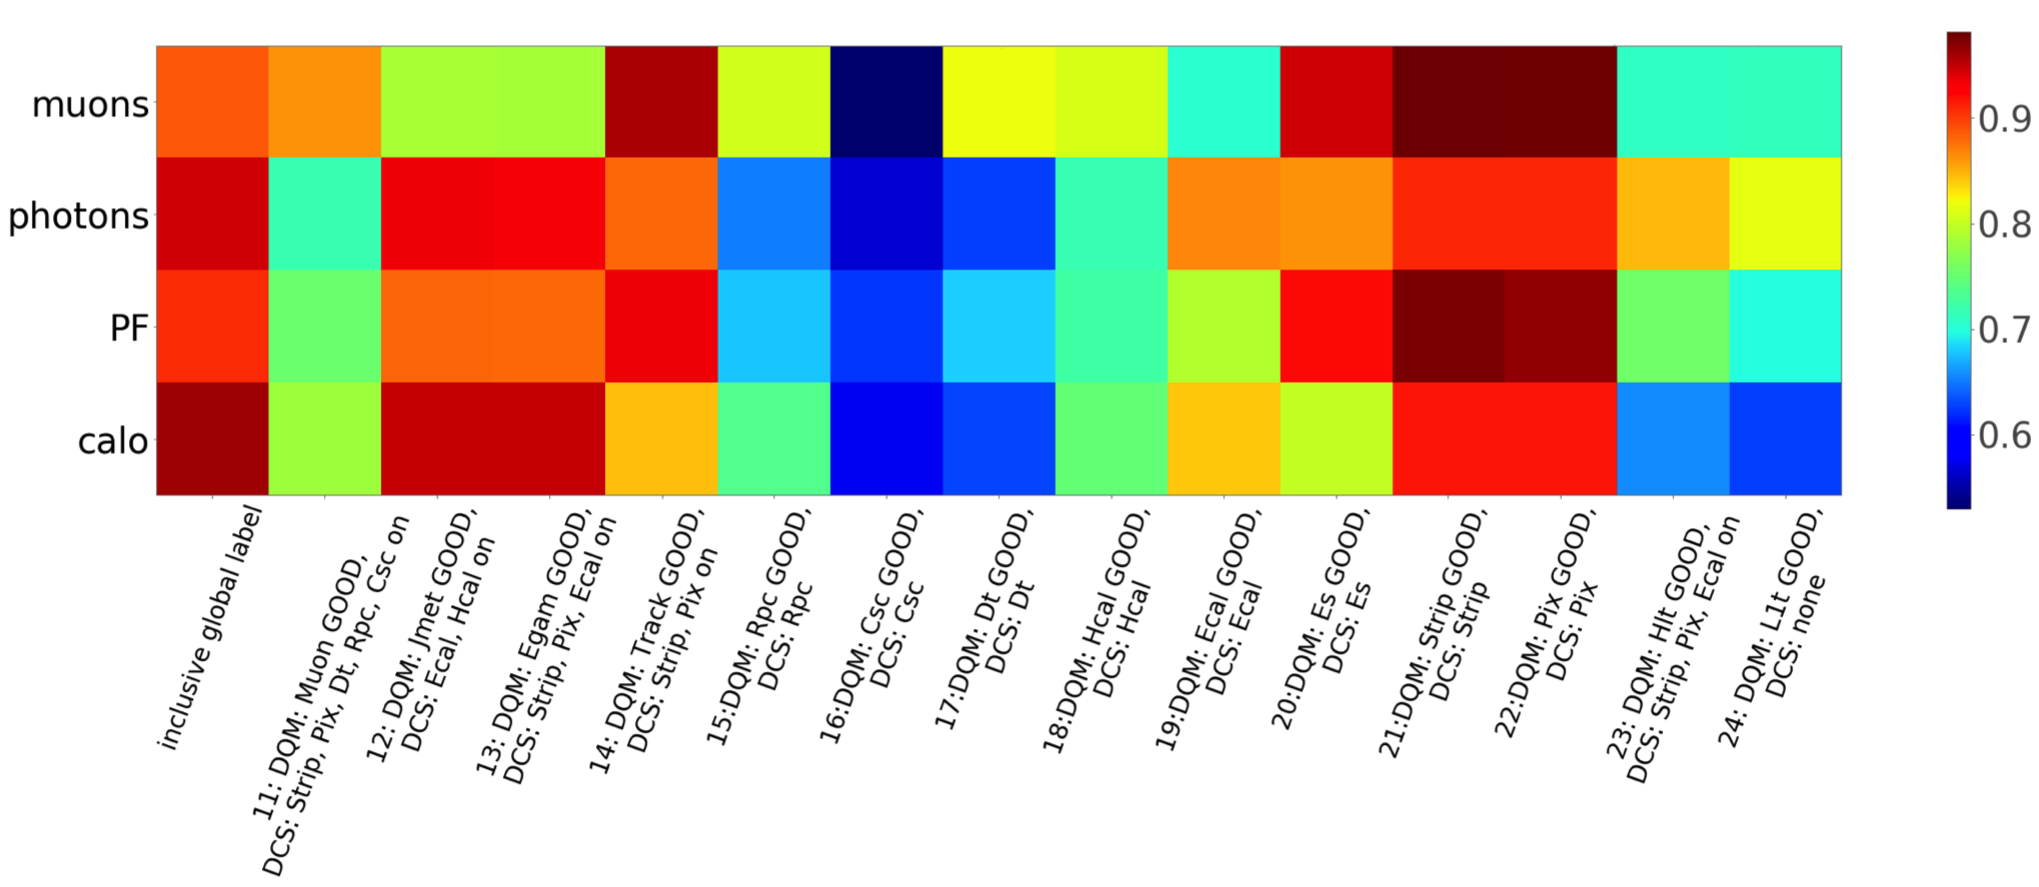
\includegraphics[width=5.5in]{figures/aucs.png}
\end{center}
\caption{\label{label}ROC AUC scores of NN branches scores against experts' labels for CMS subsystems}
\end{figure}



\section{Conclusions}
In this work, we described a deep learning approach for inferring cause of data anomalies. While developed
with the CMS experiment in mind, we use an agnostic approach which allows the straightforward
adaptation of the proposed algorithm to different experimental setups. Method shows its ability to decompose anomalies by separate channels, being applied to data collected by the CMS experiment at the LHC in 2010. While only global quality labels were used for training, we got clear correlation between sub-networks’ outputs and corresponding true subsystem labels, what proves correctness of obtained results.

\section{Acknowledgements}
The research leading to these results was partly supported by Russian Science Foundation under grant agreement N\textsuperscript{\underline{\scriptsize o}} 17-72-20127.

\section*{References}
\begin{thebibliography}{2}
\item Borisyak M, Ratnikov F, Derkach D and Ustyuzhanin A. Towards automation of data quality system for CERN CMS experiment. {\tt arXiv:1709.08607 [physics.data-an]}, September 2017

\item  Calderon A, Colling D, Huffman A, Lassila-Perini K, McCauley T, Rao A, Rodriguez-Marrero A and Sexton-Kennedy E 2015 {\it J. Phys.: Conf. Ser.} {\bf 664} 032027
\end{thebibliography}

\end{document}

